\subchapter{Measure boot time - Hardware solution}{Objective: measure
boot time with hardware}

During this lab, we will use a hardware technique to measure boot time,
from cold boot (or reset) to the instant when the first frame has been
decoded.

\section{Arduino setup}

Take the Arduino Nano board provided by your instructor. Connect it in
the middle of the breadboard provided too, so that you can connect
wires to both sides of the Arduino.

Download the 1.8.13 version of the Arduino IDE from
\url{https://www.arduino.cc/} (don't use the Arduino
package in Ubuntu 20.04, as it has issues connecting to the serial port,
even with root privileges, while the official version works without any problem).
Extract the archive in \code{/usr/local/}.

Use the provided USB cable to connect the Arduino to your PC, and start the IDE:

\begin{verbatim}
/usr/local/arduino-1.8.13/arduino
\end{verbatim}

Now, configure the IDE for your Arduino:
\begin{itemize}
\item In \code{Tools}, \code{Board}, select \code{Arduino Nano}
\item In \code{Tools}, \code{Processor}, select \code{ATmega328p} (or
      \code{ATmega328p old bootloader} if you have a Nano clone)
\item In \code{Tools}, \code{Port}, select \code{ttyUSB1} (or
      \code{ttyUSB0} if the serial line for your Bone Black board is no longer
      connected.
\end{itemize}

Now are now ready to use your Arduino board:
\begin{itemize}
\item Go to \code{Files}, \code{Examples}, \code{01. Basics} and select \code{Blink}.
      This program allows to blink the LED on the Nano.
\item Press the \code{Upload} butter and you should see the {\em sketch} work
(that's how the Arduino community call their programs).
\item You can now unplug the Arduino and plug it back. The same program
will be started automatically. Loading a program is just necessary once.
\end{itemize}

\section{7-segment display setup}

We are going to use a 7-segment display to display time elapsed since
the last time the Beagle Bone Black board was last reset.

Take the TM1637 module provided by your instructor, and insert its pins
into the breadboard at a convenient location.

Now, using breadboard wires, connect the \code{GND} pin of the Arduino to one
of the blue rails of the breadboard, then to the \code{GND} pin of the 7-segment
module. Please use blue or black wires!

Similarly, connect the \code{5V} pin of the Arduino to the red rail of
the breadboard, then to the \code{5V} pin of the module. Using red or
orange wires is recommended too.

Then, you can connect the Arduino \code{D2} pin to the \code{CLK} pin of
the module, and the \code{D3} pin to the \code{DIO} pin of the module:

\begin{center}
\includegraphics[width=0.6\textwidth]{labs/boot-time-hardware-measurement/nano-7segment.png}
\end{center}

Now, let's test your wiring by loading the sketch in
\code{~/boot-time-labs/arduino/test-7segment/}. Upload and try to run it.

Oops, a library is missing. You could have retrieved it through the
IDE's library manager (\code{Tools}, \code{Manage Libraries}), but in
this case, we absolutely need its latest version. So, go to
\url{https://github.com/Seeed-Studio/Grove_4Digital_Display},
download a zip file and extract this archive into
\code{~/Arduino/libraries/}. Rename \code{Grove_4Digital_Display-master}
to \code{Grove_4Digital_Display} (removing the \code{-master} suffix
added by GitHub, and you should be ready to go.

\section{Configuring Bone Black pins as GPIOs}

Our goal is to measure boot time with the Arduino system, in a way that
is as accurate as hardware can be, and without having to rely on a slow
device which is the serial console.

\subsection{Finding a good start signal}

A first possibility would be to watch the 3.3V VDD pins of the Bone
Black board and start counting when they go high when the board is
powered on. However, it would be cumbersome to have to power off the
board each time we wish to make a measurement.

A second possibility is to watch the state of the \code{RESET} signal.
When this pin goes from high to low, and back to high, it means that the
board starts booting. That's a good time to start counting, and doing
it after each reset is a convenient solution.

Look at the Bone Black System Reference and find which pin on the P8 or
P9 headers is used to expose the \code{SYS_RESET} line.

\subsection{Finding a free pin for the stop signal}

Look at the schematics for the 4.3" LCD. Unfortunately, no reference
manual was ever published for this cape. However, the schematics are
sufficient to find pins that are not used by the 4.3" LCD cape.

If you look for \code{Bootlin} in the Device Tree Source we provided,
you can see in the pin definitions sections that we selected pin 13 or
the P9 headers:

\begin{verbatim}
// Bootlin: use idle pin as custom GPIO
0x074 (PIN_OUTPUT | MUX_MODE7)  /* P9_13: uart4_txd_txd.gpio0_31 */
\end{verbatim}

If you look at the \code{Expansion Header P9 Pinout} table in the
Board's Reference Manual, you will see that \code{MODE7} allows to get
GPIO number 31 on P9's pin 13.

Back to the pin for \code{SYS_RESET}, there is nothing to configure to
get it. It's the only line connected to the pin.

\subsection{Wiring these pins}

We are going the good old wire wrapping technique as shown by the
instructor to hook up to pins we want to monitor, with a reliable
connection, but without any soldering.

So, take out the LCD cape, find which of its header pins are connected
to the Bone Black pins we want to monitor, and then use the wire and
tool provided by the instructor to connect to these pins, before
re-attaching the LCD cape.

On the other end of the cables, your instructor will also give you small
headers that you can plug into the breadboard holes and do some wiring
wrapping on them too.

\subsection{Pull up or pull down?}

We need to control the state of the pins we watch when they are not
driven.

For the \code{SYS_RESET} signal, we are lucky that the ATmega328p CPU
pins can be configured as pull-up, so we just need to configure them
in software without having to use our own resistors.

For our custom GPIO pin, there only one choice because we cannot use
pull-up. If we used our own resistor, we would have a 5V voltage level
coming from the Arduino, and the Beagle Bone Black is {\bf not 5V
tolerant}, as explicited in its manual. Therefore, pull-down is our only
option. As a consequence, as the Arduino just supports pull-up for
pins, we will have to use our own pull-down resistors.

Then which Arduino pins to connect to? As the Beagle Bone Black board
has a 3.3V voltage level, it's best to use the Arduino's Analog pins to
measure the voltage driven by the Bone Black with precision. We will measure a
small integer value for 0V, and about 700 (out of a 1024 maximum) for
3.3V.

So, let's use Arduino pin \code{A0} for reset, and pin \code{A1} for the
custom GPIO, adding a 1 Kohm pull-down resistor provided by your
instructor:

\begin{center}
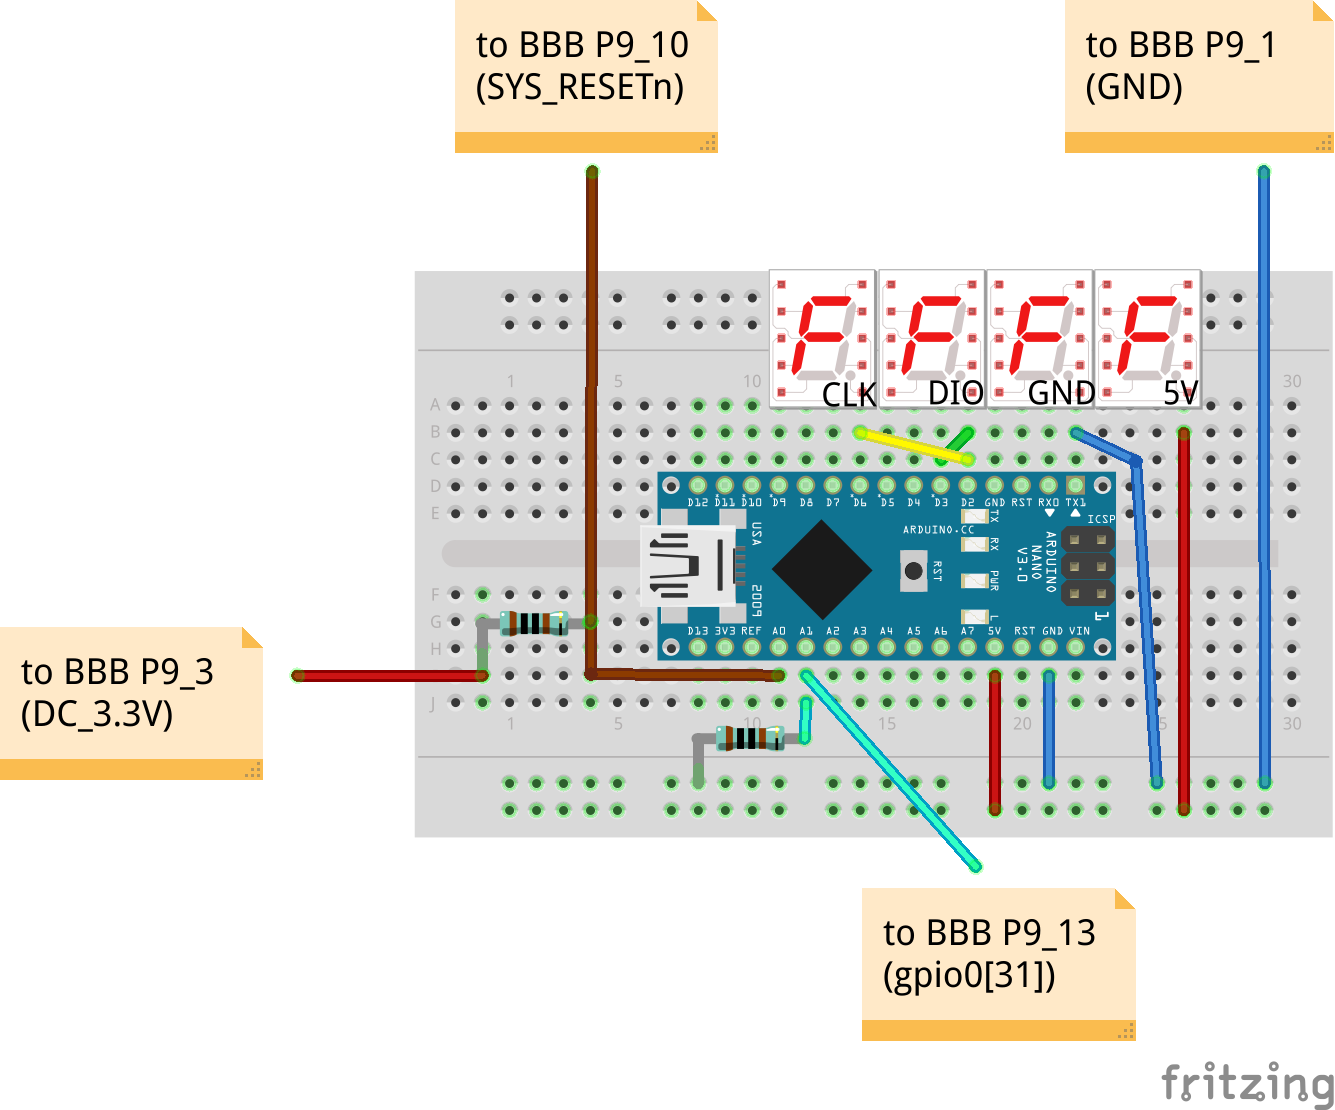
\includegraphics[width=0.7\textwidth]{labs/boot-time-hardware-measurement/nano-final.png}
\end{center}

\section{Making ffmpeg drive the custom GPIO}

Once we know how to modify \code{ffmpeg} to write to its output after
processing the first frame, it's easy to add code that configures our
custom GPIO line and drives it.

So, modify your Buildroot customizations so that you use the patch in
\code{boot-time-labs/rootfs/data/0001-ffmpeg-first-frame-completion-log-and-gpio.patc}
instead of the previously used one (look at what it does!).

Rebuild and reflash your root filesystem.

\section{Final version of the Arduino program}

We should now be able to test our full system.  Loading the sketch in
\code{~/boot-time-labs/arduino/stopwatch/}. Upload and run it.

If things don't work as expected, you can also open the Arduino Serial
Monitor (in the \code{Tools} menu), and read the pins values that
displayed there by the program.

Once the system works, is it in line with the software measurements?
Is it slightly more pessimistic as it's supposed to start counting
time a few cycles earlier?

